\section{Introduction}
\label{sec:intro}
%\begin{itemize}
%\item Why using small LM on domain specific tasks is important.
%\item How demo was used previously and show the fact that nobody has
%attempted what we are doing here (we are the first!). Give a possible reason
%why people have not used demo on small LM's before.
%\item In this paper, we design a series of experiments to show the
%effectiveness of demos on small LMs  and analyze how they are useful
%and why they are useful.
%\end{itemize}

Large language models~(LLMs) like GPT-3~\cite{gpt3,cot}~have demonstrated remarkable in-context learning capability, where the model performs few-shot learning by conditioning on a handful of
 input-output pairs~(demonstrations) without updating any parameters. Despite the impressive performance, LLMs inevitably consumes massive computation resources, which significantly hinders the 
 democratization of NLP-powered applications for public use.

Therefore, a natural question is whether in-context learning ability can be elicited from small PLMs, e.g., GPT-2~\cite{gpt2}, that are affordable to most practitioners. 
Unfortunately, it has been shown that \textit{without fine-tuning}, GPT-2 performs poorly when provided with task-specific demonstrations. For example, leveraging $64$ in-context demonstrations improves accuracy of the 175B GPT-3 on TriviaQA~\cite{triviaqa} by $6.9\%$, while the gain for 0.1B GPT-2 is marginal. 
Moreover, as the zero-shot performance of GPT-2 is already dramatically inferior than GPT-3, in-context learning seems to be even more meaningless.


In this paper, we investigate whether \textit{fine-tuned} small PLMs can benefit from in-context demonstrations. Specifically, we utilize GPT-2 as a representative small PLM and evaluate how fine-tuning affect its in-context learning ability within the scope of arithmetic problem sovling. 
We explore two different fine-tuning strategies: vanilla fine-tuning and causal language modeling~\cite{gpt2} . The former maximizes the conditional likelihood of an answer given the question on a per-sample basis, while the latter 
packs multiple training samples into a sequence and optimizes the causal language modeling objective. 

Experiment results show that adding demonstrations can drastically improve the accuracy of model fine-tuned via causal language modeling, while using demonstrations for vanilla finetuned language model doesn't bring further improvements in its accuracy. 
We also make some attempts to study whether different type of demonstrations or the order between demonstrations will affect model's accuracy. The results show that the model produces quite robust predictions regardless of the order between different demonstrations.
We hope that our observations provide some inspirations for future research on how to finetune a language model so that it can benefit from in-context demonstrations.

\begin{figure}[th]
\begin{center}
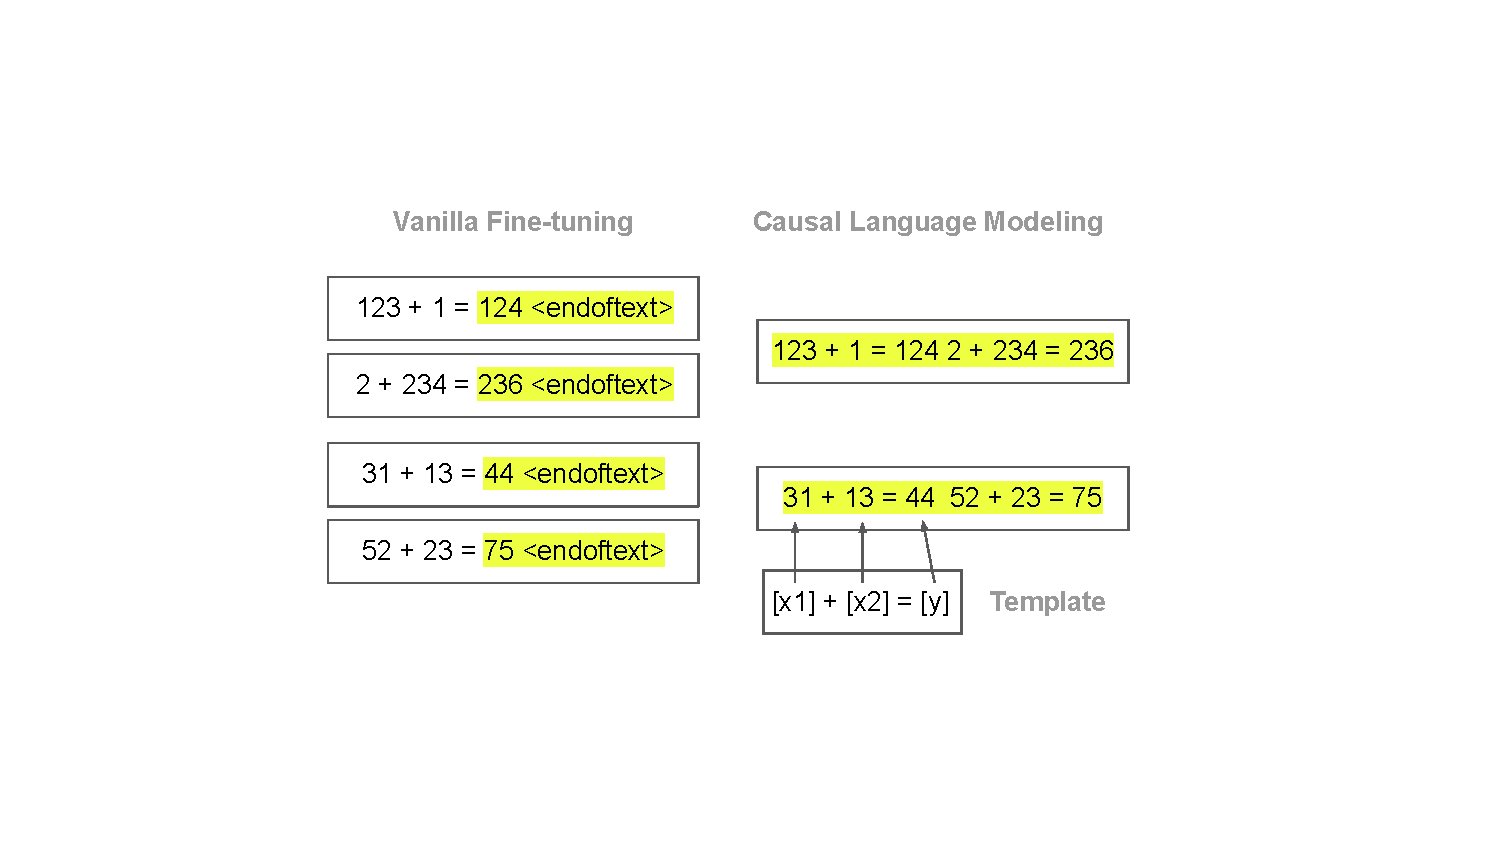
\includegraphics[width = \columnwidth]{figs/diff-vanilla-clm.pdf}
 \caption{Difference between vanilla fine-tuning and causal language modeling illustrated using an addition arithmetic example. The tokens used to calculate the loss is highlighted.}
 \label{fig:diff}
\end{center}
\end{figure}


